\documentclass{article}
\usepackage{ctex}
\usepackage{amsmath}
\usepackage{amssymb}
\usepackage{graphicx}
\usepackage{wrapfig}
\usepackage{hyperref}

\graphicspath{ {./images/} }
\title{\textbf{人工智能导论\ 四子棋\ 实验报告}}
\author{陈庆之 2021011819}

\begin{document}
	\maketitle
	
	\section{总述}
	
	四子棋是一种智力游戏。两名玩家轮流在m行n列的棋盘上落子,每次落子后棋子会落到对应列顶部。若在某次落子后己方的四枚或更多棋子在横、竖、斜向上连成直线,那么这名玩家赢得游戏。若棋盘被填满且没有任何一名玩家获胜,那么算作平局。
	
	部分大小的棋盘有必胜策略。本作业为了阻止必胜策略的应用,额外添加一不可落子点。若棋子将落入不可落子点,改为落在不可落子点正上方。若不可落子点位于列顶且其下已满,则不能在本列落子。
	
	本次作业中,我们利用\textbf{Monte-Carlo}算法进行\textbf{信心上限树搜索},实现了四子棋AI程序。在Saiblo平台上,我们提交的AI达到了95\%胜率(在偶数编号标准AI上测试)。
	
	\section{实现方法}
	
	\subsection{Monte-Carlo树搜索}
	
	人类在进行棋类游戏时通常通过归纳总结行棋,即基于经验和逻辑推导分析出各个情况的优劣,然后选择自己认可的行动。但是,简单的AI模型通常不具备完备的类人的逻辑思维能力。如果局面较为简单,程序可以利用算力优势枚举每一种可能的情况并挑选其中最好的策略,但对于绝大多数足以被称为棋类运动的游戏,这样枚举出的决策树会指数级增长,枚举的复杂度是不可接受的。
	
	Monte-Carlo算法即反其道而行之,纯粹使用统计与概率的方式行棋直至比赛结束,将随机行棋的结果记录到各个着法上,并依据随机行棋的结果统计出“最可能获胜”的着法。只要随机行棋的次数足够多,大数定律就可以保证统计的结果基本收敛到着法的好坏。
	
	具体而言,对于每个局面$state$,我们定义其奖赏(reward)为:$reward = \frac{n_{\text{win}} - n_{\text{loss}}}{n_{\text{simulation}}}$, 其中win/loss/simulation分别对应当前局面下的胜利次数、失败次数和总模拟次数。注意,我们并不关心从当前局面出发之后,接下来的行棋过程是带有策略或筛选的,还是全部或部分随机挑选着法的。只要是完成了一次模拟并获得了最终结果,我们就记录到当前局面上。换言之,每个局面的记录都会回溯到决策树的根。
	
	\subsection{UCT}
	
	\textbf{信心上限树搜索}(\textbf{U}pper \textbf{C}onfidence bounds applied to \textbf{T}rees)是Monte-Carlo树搜索的优化版本。设想存在某一步坏棋,如果下出这步棋,那么对手有一些强制着法可以在若干步内获胜或者获得巨大优势,但如果对手错过了这些强制着法,那么我方可以轻易获胜。如果纯粹地按照Monte-Carlo树的方法随机落子,那么这步坏棋会因为“大多数”后续着法都对我方有利而被错误地评估为好棋,殊不知对手只要棋艺不是太差都能让我们立刻输掉游戏。实际上,在棋类游戏中这样的情形很常见:国际象棋有句名言“胜利者是犯下倒数第二个错误的人”,即说明很多时候一着不慎就可满盘皆输。
	
	针对这种情况,我们使用了UCT算法。它的核心思路是:每个局面的评估不再只与当前局面的胜率有关,还与当前局面的模拟次数有关。形式化地,设$n$为某个局面被模拟的次数,$w$为胜利次数,则每个子局面$j$的UCT值可表示为:
	
	\begin{equation}
		UCT = \frac{w_j}{n_j} + c\sqrt{\frac{\ln{n}}{n_j}}
	\end{equation}

	其中$c$为一常数,$c$越大则程序越倾向于探索访问较少的策略(更激进,不“安于现状”)。这样就可以提升Monte-Carlo过程的广度,尽可能减少前述情况。
	
	\subsection{实现}
	
	我们的算法流程大致如下:
	
	\begin{figure}[ht]
		\centering
		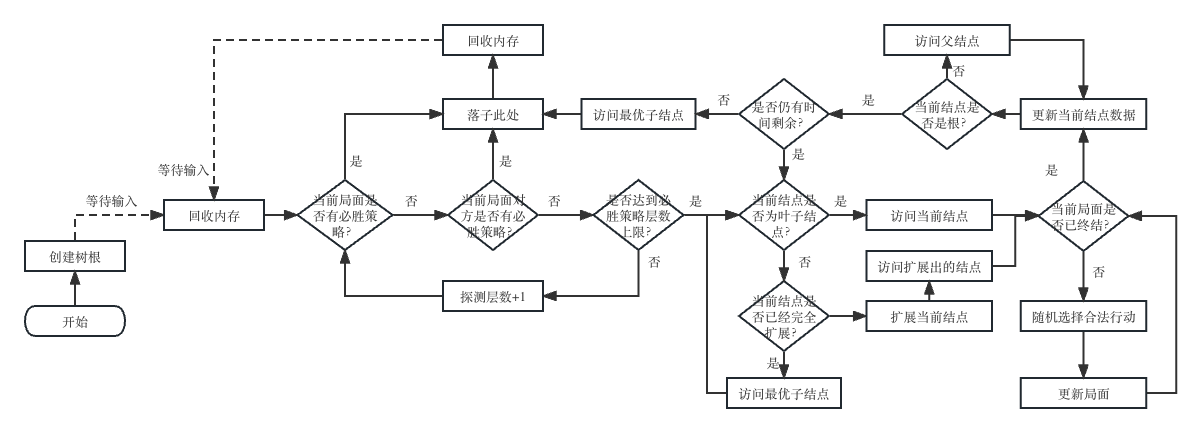
\includegraphics[width=0.9\textwidth]{procedure.png}
		\caption{四子棋算法流程}
	\end{figure}
	
	一次落子分为四个步骤:
	\begin{enumerate}
		\item 根据传入的对方的落子信息,从第一层决策树中删去无关结点;
		\item 轮流枚举若干步以内是否有自己/对方的必胜策略,若有,则直接落子在该位置\footnote{假如自己没有更快的必胜策略,那么阻止对手必胜策略的唯一方式是落在对手要落子的地方。};
		\item 从根结点开始,如果当前结点没有扩展完毕而且不是最终状态就扩展它,否则进入最好的子结点尝试扩展;
		\item 从上一步选择的结点开始,随机落子直到游戏结束,记录结果;
		\item 从上一步选择的结点开始,向上回溯到根,期间修正每个结点的reward。
	\end{enumerate}
	
	我们的决策树在不同落子之间是\textbf{继承}的。每次轮流落子之间,可以删除两层的决策树、只保留实际落子的根结点以回收存储空间。
	
	\section{参数}
	
	\subsection{搜索时间}
	
	tl; dr: 我们刻意没有用完3s时间。
	
	经过试验,我们发现Saiblo平台的评测机非常不稳定,甚至设置为搜索时间2.25s都有小概率超时(在极度繁忙的时候)。因此,我们最后决定将搜索时间定在2s。实际上,在算法实现正确的情况下,对我们这样有记忆的搜索而言相对来说不太关心2s和3s之间的常数级差别。由于UCB在无限时间下收敛到minimax算法,理论上提升这个参数能够继续提升胜率,但为了保险起见,我们没有压榨时间参数到极致。
	
	\subsection{UCT常数}
	
	UCT常数(即式子中的$c$)可以决定AI的风格。$c$越大,算法越愿意探索新的分支,但代价是搜索效率可能降低,因为有许多论胜率而言并不高的结点被重复选中。
	
	初始时我们依据经验设置此常数为0.7.之后,我们对这个常数做了若干次修改测试,但是由于初始的胜率已经达到94\%,修改后的浮动可以视为偶然误差,统计上没有显著意义(甚至无法通过单盲试验)。与本届及往届同学交流后决定就以初始的0.7作为最终提交版本中的UCT常数。
	
	\subsection{必胜策略深度}
	
	首先我们detail一下必胜策略实现方式。我们在一个预先申请好的内存空间里复制一张棋盘(就像rollout过程那样),然后遍历每一种合法的落子,判断是否是\textbf{k-必胜着法}。一个着法是一个k-必胜着法,当且仅当:
	
	\begin{enumerate}
		\item 这步着法落子后直接获胜;或者
		\item k>0, 且这步着法之后对手任意着法都不能直接获胜,且对于任意对手着法,己方都存在一个(k-1)-必胜着法。
	\end{enumerate}
	
	可以想见,搜索的时间复杂度是$O(10^n)$左右的,因此不能搜得太深,否则可能挤占Monte-Carlo的时间。在全部的测试样例上,我们尝试了k=0(即没有考虑必胜策略),1,2,3的情形:
	
	\begin{table}[h]
		\centering
		\begin{tabular}{||c|c|c|c|c||}
			\hline $k$&0&1&2&3 \\
			\hline 胜率&92&\textbf{95}&85&75\\
			\hline
		\end{tabular}
	\end{table}

	我们发现,单纯地增加必胜策略搜索层数不能有效提高胜率。我们提出两点原因:
	
	其一,搜索到3层时,可能的搜索结点数已经达到了约$10^6$个,而我们调试过程中发现3s内总Rollout次数也不过约$10^6$数量级。这就意味着过深的必胜策略搜索严重占用了Monte-Carlo主过程的时间,从而影响行棋质量。
	
	其二,在考虑多步必胜策略时,我们总是假定对手总能找到最优解。但是实际上用作测试的对手并不总能找到最优解。我们对具体对局进行分析后发现,存在这样的情形:我们已经进入一个理论必败的局面,但我们可以通过反复冲击三连棋而拖延时间。由于对手不够强,可能无法识别此时已经是一个$k$步杀局面,从而犯错。但若我们尝试直接封堵这个必胜序列从而下在某个位置后,由于四子棋\textit{垫脚石}的特性,可能反而让对手的必胜着法变得显然,诱使对手做出正确选择。因此搜索得太深也许不一定是好事。
	
	\section{结果汇报}
	
	\begin{figure}[ht]
		\centering
		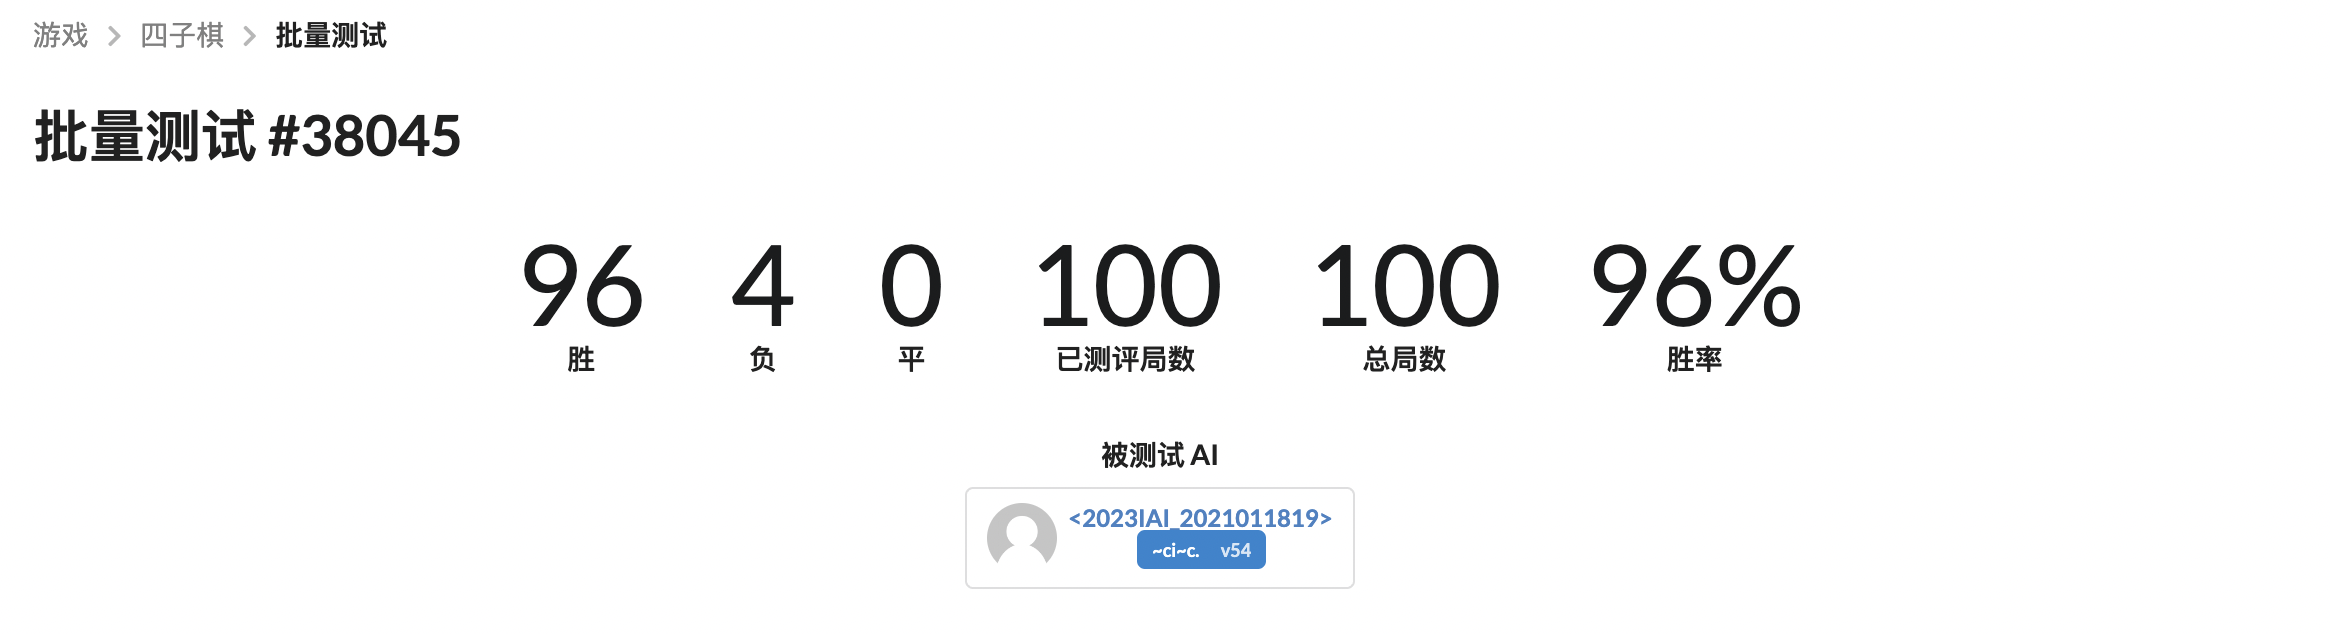
\includegraphics[width=0.9\textwidth]{result}
		\caption{v54(最终版本)样例对战结果}
	\end{figure}
	
	我们最终派遣的版本(Saiblo版本号v54)使用的参数为:2.0s搜索时间,0.7UCT常数,1层必胜策略搜索。这个版本达成了96\%胜率(96胜4负0平)。我们的benchmark是最开始实现的无必胜策略搜索的AI(Saiblo版本号v28),达成了90\%胜率(90胜10负0平)。这说明我们的优化是有效果的。
	
	\section{代码结构说明}
	
	我们没有修改给定的代码框架。
	
	我们在MyEngine.cpp/h中实现了类MyEngine和辅助类node。MyEngine是一个单例模式设计的类,用于维护棋盘信息并储存决策树。由于我们的搜索是有记忆的,仅需提供对手上一步落子即可进行决策。

\end{document}